\section{Implementierung}


\subsection{Einbindung Hardware Fußschalter}
Die Prototypen des Fußschalters von Firma Brecht wurden bereits vor Beginn dieser Arbeit erhalten und somit konnte direkt mit der Inbetriebnahme der neuen Hardware begonnen werden. Der Chipsatz des Fußschalters ist ebenfalls der PCA10056 von Nordic semiconductor, somit muss an der Software des USB-Dongles keine Änderungen vorgenommen werden. Da der Fußschalter zwar die USB-Dongle App beinhaltet, jedoch der Dongle auch als eigenständiges Produkt angeboten werden soll, muss der Code der beiden Projekt von Anfang an getrennt bleiben. Dazu muss ein neues Projektfile eingeführt werden und Abhängigkeiten zwischen den Files so gering wie möglich gehalten werden. Unvermeidbare Abhängigkeiten werden durch Compilerschalter getrennt. 

\subsubsection{Triggern des Messergebnis}
Das erste Fußschalter spezifische Feature ist, dass durch Betätigung des Fußschalters eine Messung bei Messuhren bzw. Messschiebern ausgelöst wird. Das Senden bzw. das Schreiben der Daten, die den Messvorgang in einer Messuhr auslösen, wurde dabei bereits im Zuge der Einbindung der Messuhr implementiert. Dieser Vorgang muss nun durch das Betätigen des Fußschalters ausgelöst werden. Dazu muss in einem ersten Schritt analysiert werden in welcher Form und an welchen Pin das Signal genau vorliegt und wie es abgegriffen werden kann.  

\subsubsection{Energie Management}
Wenn der Fußschalter nicht über USB mit einer Stromquelle verbunden ist, bekommt er den benötigten Strom von dem fest eingebauten Akku. Um diesen nicht unnötig zu belasten, soll der Fußschalter nach einer gewissen Zeit so weit wie möglich heruntergefahren werden.  
In der bestehenden Anwendung ist bereits ein Energiemanagement vorhanden, dieses schaltet den BLE-Chip nach einiger Zeit der Inaktivität aus. Der Chip der Anwendung verbraucht nur wenig Strom. Daher soll nach einer gewissen Zeit der Innaktivität die Verbindungen getrennt werden, Scanning und Advertising gestoppt werden, damit das Softdevice ausgeschaltet werden kann. Durch Betätigung des Fußtasters wird das Softdevice wieder gestartet und die Messmittel erneut verbunden. Wenn USB verbunden ist, sollen keine Energiesparmaßnahmen getroffen werden. 

Nach ersten Tests zeigt sich jedoch das Problem, dass bei der Hardware des Fußschalters, der Akku auf der Datenleitung des USBs liegt. Dadurch wird in der Anwendung nicht wie bei dem EvalBoard die Events für USB connected und USB disconnect erhalten. Daher muss am Fußschalter geringfügige Hardwareänderungen durchgeführt. Dabei wird die Eingangsspannung bereits vorher abgegriffen und auf den PIN des Fußtasters gelegt. Der Fußtaster erhält einen unbelegten PIN. Mit einem ADC wird dann überprüft, ob eine Spannung auf diesem PIN anliegt.

\subsubsection{Inbetriebnahme LED}
Auf dem Board des Fußschalters befindet sich eine LED die durch einen Lichtkanal nach außen hin durch das Gehäuse sichtbar gemacht wird und die dazu benutzt werden soll den internen Zustand des Geräts darzustellen. Folgende Zustände sollen abgebildet werden: 

\begin{table}[H]
	\centering
	\begin{tabular}[H]{l|l}
		Zustand & LED-Farbe \\
		\hline
		Gerät im Sleep Modus & Aus \\
		\hline
		Alle zu verbindenden Geräte verbunden & Blau \\
		\hline
		Min. ein Gerät verbunden, es wird nach den fehlenden Geräten gescannt & Blau blinkend \\
		\hline
		Kein Gerät verbunden, Scanning inaktiv & Grün \\
		\hline
		Kein Gerät verbunden, Scanning aktiv & Grün blinkend \\
		\hline
		MSC-Schreibvorgang detektiert & Gelb \\
		\hline
		Min. ein Konfigurationsfile nicht gefunden & Rot \\
		\hline
		Fehler in den Konfigurationsfiles & Rot blinkend \\
	\end{tabular}
	\caption{LED-Zustände}
\end{table}


\subsection{Messmodi}
Sowohl der Fußschalter als auch der USB-Dongle sollen in mehreren verschiedenen Operationsmodi laufen können. Dieser wird in einer zusätzlichen globalen Konfigurationsdatei spezifiziert. Zum Zeitpunkt der Implementierung der USB-App war die App die oberste Abstraktionsschicht aller USB-Funktionalität. Das ist mit Einführung der Fußschalter Funktionalitäten nicht mehr der Fall. Daher bedarf es einer neuen Abstraktionsschicht, die über USB- und Fußschalterapp und die Funktionalitäten beider dirigiert. Dadurch können die Operationsmodi programmatisch getrennt werden, sodass bestimmte Schritte des Initialisierungsprozesses, wie das Einlesen der Konfigurationsdatei der zu verbindenden Geräte, in einem Modus wie HID einzelnes Zeichen nicht ausgeführt werden.

\begin{figure}[H] 
	\centering
	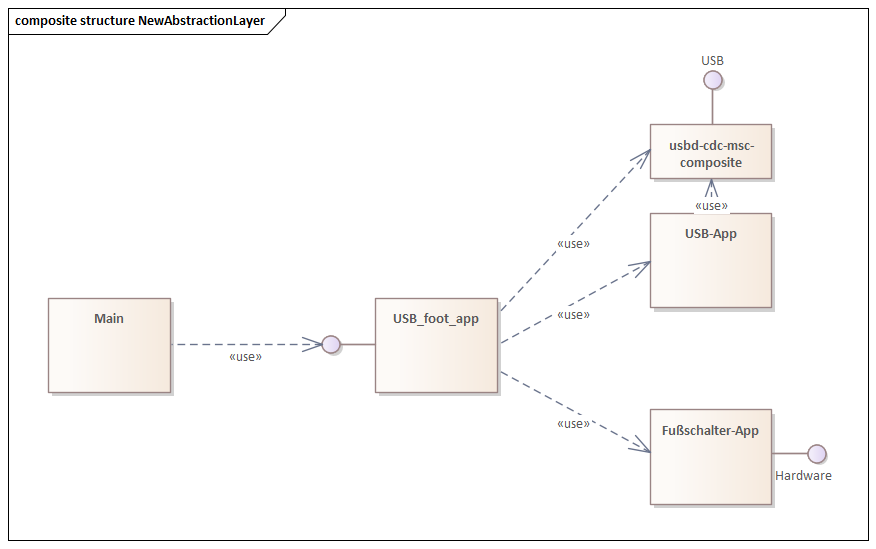
\includegraphics[width=\textwidth]{figures/NewAbstractionLayer.png}
	\caption{Neue Abstraktionsschicht}
\end{figure}

\subsubsection{USB-HID}
Ein Feature, das sowohl für die USB-App als auch für den Fußschalter implementiert werden soll, ist das Human Interface Device (HID). In diesem Modus gibt die Anwendung die Messergebnisse nicht mehr über den virtuellen COM-Port aus, sondern ist über USB als Tastatur mit Computer verbunden und gibt die Zahlen des Ergebnisses als Tastendrücke, gefolgt von einem konfigurierbaren Terminierungszeichen, ein. Dadurch können Messungen einfach in Excel oder einem Texteditor aufgefangen werde. 

In einem ersten Schritt wird grundsätzlich die Funktionalität und das Messergebnis zusätzlich zur Ausgabe über den virtuellen COM-Port ausgegeben. Dies ist eine Vorbereitung für die Implementierung der verschiedenen Operationsmodi. 

\subsubsection{BLE-HID}
Ein weiterer Modus, in dem der Fußschalter arbeiten soll, ist HID über BLE. Das bedeutet, dass sich der Fußschalter als Tastatur im kabellosen Zustand präsentieren kann und wie bei HID über USB die Messergebnisse als Tastatur Tastendrücken in einen Editor oder Excel eintippt. Dazu muss das Gerät nun zusätzlich zur Central Rolle in der Peripheral Rolle agieren. Dazu muss einerseits das Advertising korrekt konfiguriert werden und in den bestehenden Code des Peripheral Verbindungsaufbaus, die Fußschalter Applikation eingebunden werden. Für das eigentliche Schreiben des Messergebnisses über BLE wird gibt es bereits bestehenden Funktionen und diese müssen nur in der Fußschalter Applikation aufgerufen werden. Erste Tests zeigen, dass die Geschwindigkeit der Übertragung, einerseits der Dauer bis angefangen wird das Messergebnis zu schreiben und anderseits wie schnell die einzelnen Tastendrücke erfolgen, stark von USB oder einen mitlaufenden Debugger beeinträchtigt wird. Beides sollte im eigentlichen Anwendungsfall dieses Modus nicht vorhanden sein. 

\subsubsection{BLE-Windows-App}
Der letzte Modus, in dem der Fußschalter agieren soll, ist als ein an die HCT-Windows-App angebundenes Gerät. Dabei soll das Signal der Betätigung des Tasters als eine HCT-Nachricht an die Windows-App gesendet werden, welchen dann ein Messergebnis bei den mit ihr verbundenen Messgeräten triggert. Dazu muss ein HCT-Model für den Fußschalter geschaffen werden. Das Model stellt folgende Werte bereit:
\begin{itemize}
	\item Device Class
	\item Protocol type, version 
	\item Version of Hardware, Software, BLE
	\item Battery level, status
	\item Reset 
\end{itemize}

Werte des Config.ini Konfigurationsfiles:
\begin{itemize}
	\item Operating Mode 
	\item CDC protocol 
	\item HID Keyboard Language ID 
	\item HID data set seperator 
	\item HID number seperator
	\item HID single key 
\end{itemize}

Für die Übertragung des eigentlichen Signals, dass der Fußschalter betätigt wurde, muss eine HCT-Charakteristik angelegt werden, auf welche die HCT-Windows-App sich subscriben kann. Über diese Charakteristik wird sie dann über die Betätigung des Tasters notifiziert. Im Advertising muss sich der Fußschalter dann nicht als Tastatur, sondern als HCT-Fußschalter erkenntlich zeigen. Dazu  


